\documentclass[14pt]{beamer}
\usetheme{Warsaw}
\usecolortheme{beaver}
\usefonttheme{professionalfonts}

\input{../../preamble}
\usepackage{amscd,amsmath,amssymb,amsthm,graphicx}
%\usepackage[mathscr]{eucal}
\usepackage{paralist}
\usepackage{tabto}
\usepackage[normalem]{ulem}
\usepackage{tikz}
\usepackage{tkz-euclide}
\usetkzobj{all}

% % % % % % % % % %
\title[Cal I S2015]{MATH 2554 (Calculus I)}
\subtitle{}
\author[Wheeler]{Dr. Ashley K. Wheeler}
\institute{University of Arkansas}
\date{\today}
\logo{}

% % %
\begin{document}
\maketitle

% % %
\begin{frame}
\frametitle{Table of Contents}
\tableofcontents
\end{frame}

% % % % % % % % % % Mon 16 Mar 2015

% % %
\begin{frame}
\section[Week 10]{Week 10: 16-20 March}
\frametitle{Monday 16 March (Week 10)}
\small
\begin{itemize}
\item make-up midterms... almost graded.  You will find out about the curve this week.
\item Friday sub: Questions?
\item Quiz \#8 due Tues 17 Mar 	
\item Quiz \#9 handed out this Thurs, due Tues 31 Mar.  Covers $\oint 4.1-4.2$ DON'T WAIT TILL LAST MINUTE
\item Quiz \#10 in class Tues 31 Mar on $\oint 4.4$
\item Exam \#3 Friday 3 April -- expect up to $\oint 4.5$
\end{itemize}
\end{frame}

% % %
\begin{frame}
\frametitle{CEA REQUEST}
\footnotesize {\bf
A student in this class requires a note-taker. If you are willing to upload your notes and plan to attend class on a REGULAR basis, please sign up via the CEA Online Services on the Center for Educational Access (CEA) website http://cea.uark.edu. On the CEA Online Services login screen, click on ``Sign Up as a Note-taker". At the end of the semester you will receive verification of 48 community service hours OR a \$50 gift card for providing class notes. All interested students are encouraged to sign up; preference may be given to volunteers seeking community service in an effort engage U of A students in community service opportunities. Please contact the Center for Educational Access at ceanotes@uark.edu if you have any questions.}
\end{frame}

% % %
\begin{frame}
\subsection[$\oint 4.2$ What Derivatives Tell Us]{$\oint 4.2$ What Derivatives Tell Us}
\frametitle{$\oint 4.2$ What Derivatives Tell Us}
\begin{dfn} Suppose a function $f$ is defined on an interval $I$.
\begin{itemize}
\item We say that $f$ is {\bf increasing} on $I$ if $f(x_2)>f(x_1)$ whenever $x_1$ and $x_2$ are in $I$ and $x_2 > x_1$.
\item We say that $f$ is {\bf decreasing} on $I$ if $f(x_2)<f(x_1)$ whenever $x_1$ and $x_2$ are in $I$ and $x_2 > x_1$.
\end{itemize}
\end{dfn}
\end{frame}

% % %
\begin{frame}
\frametitle{\small How is it related to the derivative?}
%\small
Suppose $f$ is continuous on an interval $I$ and differentiable at every interior point of $I$.

\vspace{1pc}
\begin{itemize}
\item If \alert{$f^{\prime}(x)>0$} for all interior points of $I$, then $f$ is \alert{increasing} on $I$.

\vspace{1pc}
\item If \alert{$f^{\prime}(x)<0$} for all interior points of $I$, then $f$ is \alert{decreasing} on $I$.
\end{itemize}
\end{frame}

% % %
\begin{frame}%[t]
\frametitle{}
\begin{ex} Sketch a function that is continuous on $(-\infty,\infty)$ that has the following properties:

\begin{itemize}
\item $f^{\prime}(-1)$ is undefined;

\vspace{1pc}
\item $f^{\prime}(x)>0$ on $(-\infty,-1)$;

\vspace{1pc}
\item $f^{\prime}(x)<0$ on $(-1,\infty)$.
\end{itemize}
\end{ex}
\end{frame}

% % %
\begin{frame}%[t]
\frametitle{}
\begin{ex} Find the intervals on which
$$f(x)=3x^3-4x+12$$
is increasing and decreasing.
\end{ex}
\end{frame}

% % %
\begin{frame}
\frametitle{First Derivative Test}
\footnotesize
Suppose that $f$ is continuous on an interval that contains a critical point $c$ and assume $f$ is differentiable on an interval containing $c$, except perhaps at $c$ itself.

\begin{itemize}
\item If $f^{\prime}$ \alert{changes sign} from positive to negative as $x$ increases through $c$, then $f$ has a {\bf local maximum} at $c$.

\vspace{0.5pc}
\item If $f^{\prime}$ \alert{changes sign} from negative to positive as $x$ increases through $c$, then $f$ has a {\bf local minimum} at $c$.

\vspace{0.5pc}
\item If $f^{\prime}$ does not change sign at $c$ (from positive to negative or vice versa), then $f$ has {\bf no} local extreme value at $c$.
\end{itemize}

\alert{{\bf NOTE:} The First Derivative Test does NOT test for increasing/decreasing, only local max/min.}  Use it on critical points. 
\end{frame}

% % %
\begin{frame}%[t]
\frametitle{}
\begin{exe} If $f(x)=2x^3+3x^2-12x+1$, identify the critical points on the interval $[-3,4]$, and use the First Derivative Test to locate the local maximum and minimum values.  What are the absolute max and min? \end{exe}
\end{frame}

% % %
\begin{frame}
\frametitle{\small Absolute extremes on any interval}
\small
The Extreme Value Theorem (cf., Section 4.1) stated that we were guaranteed extreme values \alert{only on closed intervals}.  

\vspace{0.5pc}
\alert{However:}  Suppose $f$ is continuous on an interval $I$ that contains only one local extremum at $(x=)c$.

\begin{itemize}
\item If it is a local minimum, then $f(c)$ \alert{is} the absolute minimum of $f$ on $I$.

\vspace{0.5pc}
\item If it is a local maximum, then $f(c)$ \alert{is} the absolute maximum of $f$ on $I$.
\end{itemize}
\end{frame}

% % %
\begin{frame}
\frametitle{\small Derivative of the derivative tells us:}
\small 
Just as the first derivative $f^{\prime}$ told us whether the function $f$ was increasing or decreasing, the second derivative $f^{\prime\prime}$ also tells us whether $f^{\prime}$ is increasing or decreasing.

\begin{dfn} Let $f$ be differentiable on an open interval $I$.
\begin{itemize}
\item If $f^{\prime}$ is increasing on $I$, then $f$ is {\bf concave up} on $I$.
\item If $f^{\prime}$ is decreasing on $I$, then $f$ is {\bf concave down} on $I$.
\end{itemize}
\end{dfn}

\begin{dfn} If $f$ is continuous at $c$ and $f$ changes concavity at $c$ (from up to down, or vice versa), then $f$ has an {\bf inflection point} at $c$. \end{dfn}
\end{frame}

% % %
\begin{frame}
\frametitle{\small Test for Concavity}
Suppose that $f^{\prime\prime}$ exists on an interval $I$.

\begin{itemize}
\item If $f^{\prime\prime}>0$ on $I$, then $f$ is \alert{concave up} on $I$.

\vspace{0.5pc}
\item If $f^{\prime\prime}<0$ on $I$, then $f$ is \alert{concave down} on $I$.

\vspace{0.5pc}
\item If $c$ is a point of $I$ at which $f^{\prime\prime}(c)=0$ and $f^{\prime\prime}$ changes signs at $c$, then $f$ has an \alert{inflection point} at $c$.
\end{itemize}
\end{frame}

% % %
\begin{frame}
\frametitle{\small Second Derivative Test}
Suppose that $f^{\prime\prime}$ is continuous on an open interval containing $c$ with $f^{\prime}(c)=0$.

\begin{itemize}
\item If $f^{\prime\prime}(c)>0$, then $f$ has a \alert{local minimum} at $c$.

\vspace{0.5pc}
\item If $f^{\prime\prime}(c)<0$, then $f$ has a \alert{local maximum} at $c$.

\vspace{0.5pc}
\item If $f^{\prime\prime}(c)=0$, then the test is inconclusive.
\end{itemize}

\vspace{1pc}
{\bf See the Recap of Derivative Properties (Figure 4.36 on p.\ 242) for a summary.}
\end{frame}

% % %
\begin{frame}
\frametitle{HW from Section 4.2}
Do problems 11--35 odd, 47--61 odd, 67 (pp.\ 243--245 in textbook)
\end{frame}

% % % % % % % % % % Wed 18 Mar 2015

% % %
\begin{frame}
\frametitle{Wednesday 18 March (Week 10)}
\small
\begin{itemize}
\item make-up midterms... almost graded.  You will find out about the curve this week.
\item Quiz \#9 handed out this Thurs, due Tues 31 Mar.  Covers $\oint 4.1-4.2$ DON'T WAIT TILL LAST MINUTE
\item Quiz \#10 in class Tues 31 Mar on $\oint 4.4$
\item Exam \#3 Friday 3 April -- expect up to $\oint 4.5$
\end{itemize}
\end{frame}

% % %
\begin{frame}%[t]
\frametitle{\small $\oint 4.2$, cont.}
\begin{exe}
Let $f(x)=2x^3-6x^2-18x.$

\begin{itemize}
\item[1.] Determine the intervals on which $f$ is concave up or down, and identify any inflection points.

\vspace{0.5pc}
\item[2.] Locate the critical points, and use the Second Derivative Test to determine whether they correspond to local minima or maxima, or whether the test is inconclusive.
\end{itemize}
\end{exe}
\end{frame}

% % %
\begin{frame}
\subsection[$\oint 4.3$ Graphing Functions]{$\oint 4.3$ Graphing Functions}
\frametitle{$\oint 4.3$ Graphing Functions}
\footnotesize
{\bf Graphing Guidelines:}
\begin{itemize}
\item[1.] Identify the domain or interval of interest.
\item[2.] Exploit symmetry.
\item[3.] Find the first and second derivatives.
\item[4.] Find critical points and possible inflection points.
\item[5.] Find intervals on which the function is increasing or decreasing, and concave up/down.
\item[6.] Identify extreme values and inflection points.
\item[7.] Locate vertical/horizontal asymptotes and determine end behavior.
\item[8.] Find the intercepts.
\item[9.] Choose an appropriate graphing window and make a graph.
\end{itemize}
\end{frame}

% % %
\begin{frame}
\begin{exe} According to the graphing guidelines, sketch a graph of 
\[f(x)=\frac{x^2}{x^2-4}.\]
\end{exe}
\end{frame}

% % %
\begin{frame}
\frametitle{HW from Section 4.3}
Do problems 7, 9, 13--19 odd, 23, 29, 43, 45 (pp.\ 254--255 in textbook)
\end{frame}

% % % % % % % % % % Fri 20 Mar 2015

% % %
\begin{frame}
\frametitle{Friday 20 March (Week 10)}
\small
\begin{itemize}
\item Quiz \#9 handed out this Thurs, due Tues 31 Mar.  Covers $\oint 4.1-4.2$ DON'T WAIT TILL LAST MINUTE
\item Quiz \#10 in class Tues 31 Mar on $\oint 4.4$
\item Exam \#3 Friday 3 April -- covers up to $\oint 4.5$
\end{itemize}
\end{frame}

% % %
\begin{frame}
\subsection[$\oint 4.4$ Optimization Problems]{$\oint 4.4$ Optimization Problems}
\frametitle{$\oint 4.4$ Optimization Problems}
\small
In many scenarios, it is important to find a maximum or minimum value under given constraints.  Given our use of derivatives from the previous sections, optimization problems follow directly from what we have studied.
\end{frame}

% % %
\begin{frame}
\frametitle{}
\small
\begin{que} Given all nonnegative real numbers $x$ and $y$ between 0 and 50 such that their sum is 50 (i.e., $x+y=50$), which pair has the maximum product? \end{que}

\vspace{2pc}
This is a basic optimization problem.  In this problem, we are given a \alert{\bf constraint} ($x+y=50$) and asked to maximize an \alert{\bf objective function} ($A=xy$).
\end{frame}

% % %
\begin{frame}
\frametitle{}
\small
The first step is to express the objective function $A=xy$ in terms of a \alert{single variable} by using the constraint:
\[y=50-x \implies A(x)=x(50-x).\]

\vspace{2pc}
To maximize $A$, we find the critical points:
\[A^{\prime}(x)=50-2x\ \text{which has a critical point at}\ x=25.\]
\end{frame}

% % %
\begin{frame}
\frametitle{}
Since $A(x)$ has domain $[0,50]$, to maximize $A$ we evaluate $A$ \alert{at the endpoints of the domain and at the critical point}:
\[A(0)=A(50)=0\ \text{and}\ A(25)=625.\]

\vspace{2pc}
So 625 is the maximum value of $A$ and $A$ is maximized when $x=25$ (which means $y=25$).
\end{frame}

% % %
\begin{frame}
\frametitle{\small Essential Feature of Optimization Problems}
\small
All optimization problems take the following form:
\begin{center}
\alert{\it What is the maximum (or minimum) value of an objective function subject to the given constraint(s)?}
\end{center}

\vspace{2pc}
Most optimization problems have the same basic structure as the previous problem:  An objective function (possibly with several variables and/or constraints) with methods of calculus used to find the maximum/minimum values.
\end{frame}

% % %
\begin{frame}
\frametitle{}
\small
\begin{exe} Suppose you wish to build a rectangular pen with two interior parallel partitions using 500 feet of fencing.  What dimensions will maximize the total area of the pen?
\begin{center}
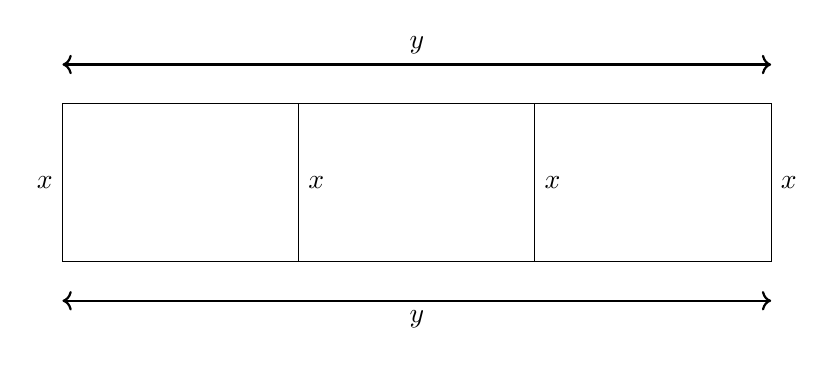
\begin{tikzpicture}
\draw (0,0) -- (3,0) 
   -- (3,2) node[midway,right] {$x$}
	 -- (0,2)
   -- (0,0) node[midway,left] {$x$};
\draw (3,0) -- (6,0)
	 -- (6,2) node[midway,right] {$x$}
	 -- (3,2)
	 -- (3,0);
\draw (6,0) -- (9,0)
	 -- (9,2) node[midway,right] {$x$}
	 -- (6,2)
	 -- (6,0);
\draw [<->] [thick] (0,-0.5) -- (9,-0.5) node[midway,below] {$y$};
\draw [<->] [thick] (0,2.5) -- (9,2.5) node[midway,above] {$y$};
\end{tikzpicture}
\end{center}
\end{exe}
\end{frame}

% % %
\begin{frame}
\small
By the picture, $2y+4x=500$ which implies $y=-2x+250$.  We are maximizing $A=xy$.  So write
\[A(x)=x(-2x+250)=-2x^2+250x.\]

Taking the derivative, $A^{\prime}(x)=-4x+250=0$, $A$ has a critical point at $x=62.5.$
\end{frame}

% % %
\begin{frame}
\footnotesize
From the picture, since we have $500$ ft of fencing available we must have $0 \le x \le 125$.  To find the max we must examine the points $x=0,62.5,125$:
\[A(\alert{0})=A(\alert{125})=0\text{ and }A(\alert{62.5})=7812.5\]

\vspace{1pc}
We see that 
\[\boxed{\text{the maximum area is}\ 7812.5\ \text{ft}^2.}\]
The pen's dimensions (answer the question!) are $\boxed{x=62.5\ \text{ft}}$ and 
\[\boxed{y=-2(62.5)+250=125\ \text{ft}.}\]
\end{frame}

% % %
\begin{frame}
\frametitle{\small Guidelines for Optimization Problems}
\footnotesize
\begin{itemize}
\item[1.] \alert{READ THE PROBLEM} carefully, identify the variables, and organize the given information with a picture.
\item[2.] Identify the objective function (i.e., the function to be optimized).  Write it in terms of the variables of the problem.
\item[3.] Identify the constraint(s).  Write them in terms of the variables of the problem.
\item[4.] Use the constraint(s) to eliminate all but one independent variable of the objective function.  
\item[5.] With the objective function expressed in terms of a single variable, find the interval of interest for that variable.
\item[6.] Use methods of calculus to find the absolute maximum or minimum value of the objective function on the interval of interest.  If necessary, \alert{check the endpoints}.
\end{itemize}
\end{frame}

% % %
\begin{frame}%[t]
\frametitle{}
\small
\begin{exe} An open rectangular box with square base is to be made from $48\ \text{ft}^2$ of material.  What dimensions will result in a box with the largest possible volume? \end{exe}

\vspace{1pc}
\begin{exe} Find the dimensions of the rectangle of largest area which can be inscribed in the closed region bounded by the $x$-axis, $y$-axis, and the graph of $y=8-x^3$. \end{exe}
\end{frame}

% % %
\begin{frame}
\frametitle{HW from Section 4.4}
Do problems 5--13 all, 18--20 all, 26 (pp.\ 261--263 in textbook)
\end{frame}


\begin{comment}
\end{comment}

\end{document}